\section{Segment Routing}

RFC 8402: \url{https://datatracker.ietf.org/doc/html/rfc8402}

\vspace{5mm}
\emph{``Segment Routing (SR) leverages the source routing paradigm.  A node 
   steers a packet through an ordered list of instructions, called 
   segments.  A segment can represent any instruction, topological or 
   service based.  A segment can have a semantic local to an SR node or 
   global within an SR domain.  SR provides a mechanism that allows a 
   flow to be restricted to a specific topological path, while 
   maintaining per-flow state only at the ingress node(s) to the SR 
   domain.''}

\begin{itemize}
    \item Prefix-SIDs are 
    \item Adjacency-SIDs are labels with the format 24NXY for the N-th adjacency from x $ \rightarrow $ y
    \item LDP/RSVP/BGP labels are in the range  [90000 - 99999]
\end{itemize}

\vspace{5mm}
\textbf{Source Routing}: The entire path is calculated as a \emph{Segment List} by the source router, or received by a PCE (Path Computation Element). 
The rest of the network only executes these encoded instructions, there is no per-flow state information. 

\vspace{5mm}
\textbf{Segment:} An instruction to the processing device on how to forward the packet. The Segment-ID can be encoded as an MPLS label or an IPv6 and is usually associated
either with a destination prefix, a local interface or a local service. In combination, a list of segments specifies the entire path a packet is supposed to take.

\vspace{5mm}
\textbf{Local Segment:} Only the node that originates this segment understands the associated instruction.

\vspace{5mm}
\textbf{Global Segment:} Each node in the SR Domain understands the associated instruction and installs it in its forwarding table.

Default label range [16000- 23999] is called SRGB / Segment Routing Global Block.

\vspace{5mm}
\textbf{Instruction: } can be one of the following three.

\noindent
PUSH -- insert segment(s) at the packet head and set first as active

\noindent
CONTINUE -- active segment is not completed and remains active

\noindent
NEXT -- active segment is completed, make next item in SID list active

\subsection{IGP Extensions}

See also: \href{https://www.segment-routing.net/tutorials/2016-09-27-segment-routing-igp-control-plane/}{Segment Routing IGP Control Plane on segment-routing.net}

\vspace{5mm}
The following segment types are based on on IGP routing information. The usual topology updates with added SID information are distributed by the IGP protocol within the SR-Domain.
Prefix-to-SID mapping server 

SR for IS-IS supports TLV extensions of the routing protocol -- additional Information transmitted via Link State Packets (LSP)

SR for OSPF is implemented by adding new Types of LSA (Link State Advertisements).

Metric-style wide must be applied for the routing protocol configuration in order to support SR capabilities.

\vspace{5mm}
Some sub-TLVs supported are
\begin{itemize}
    \item SR Capability: IS-IS router Capability
    \item Prefix-SID: Extended IP Reachability
    \item Prefix-SID: IPv6 IP Reachability
    \item Prefix-SID: SID/Label Binding
    \item Adjacency-SID: Extended IS Reachability
    \item LAN-Adjacecny-SID: Extended IS Reachability
\end{itemize}


\subsubsection{IGP Prefix Segment \emph{(global)}}
Shortest path to any known IGP network prefix. 
ECMP-aware. 
Global Segment, Label identified as 16000 + Index.
Distributed by ISIS/OSPF.
Prefix SID is domain-wide unique, assigned manually to the loopback address of each node.
\textbf{Algorithm ID} specifies the method of choosing a path. Default is 0, shortest path.

To ensure uniqueness of Prefix-SIDs, only one can be associated with each Prefix/Algorithm combination.

Example:

\noindent
\ttfamily
1.1.1.1/32 prefix-SID 1001 for algorithm 0 \\ 
1.1.1.1/32 prefix-SID 2001 for algorithm 1 \\
\rmfamily

\begin{figure}
    \centering
    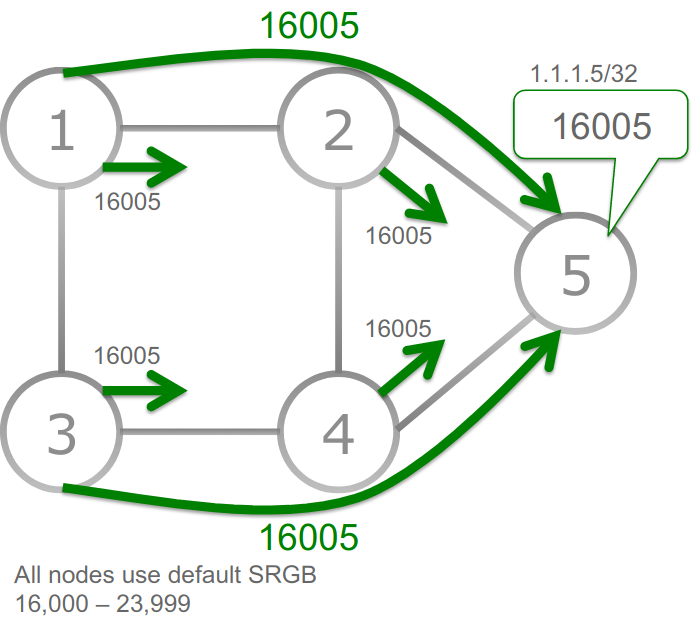
\includegraphics[width=80mm]{sr-prefix-sid.png}
    \caption{IGP Prefix Segment}
\end{figure}

\vspace{5mm}
\noindent
A Prefix Segment can be of two different types
\begin{itemize}
    \item Node Segment \\
    Associated with a /32 prefix which is a node address. \\
    Sets \textbf{N-Flag} in Segment ID.
    \item Anycast Segment \\
    Associated with an anycast prefix, which routes to the geographically closest out of a group of hosts. \\
    N-Flag is unset! \\ 
    Macro-Engineering: can be used to steer traffic via specific region, or make it pass some router performing special network functions. \\
    Offers ECMP load balancing and high availability.
\end{itemize}

\subsubsection{Adjacency Segment \emph{(local)}}
Unidirectional Adjacency, traffic is steered explicitly over an interface / link. 
Overrides shortest path routing decisions.
SID list contains node prefix first, then Adjacency-ID. 
Distributed by ISIS/OSPF.

\begin{figure}
    \centering
    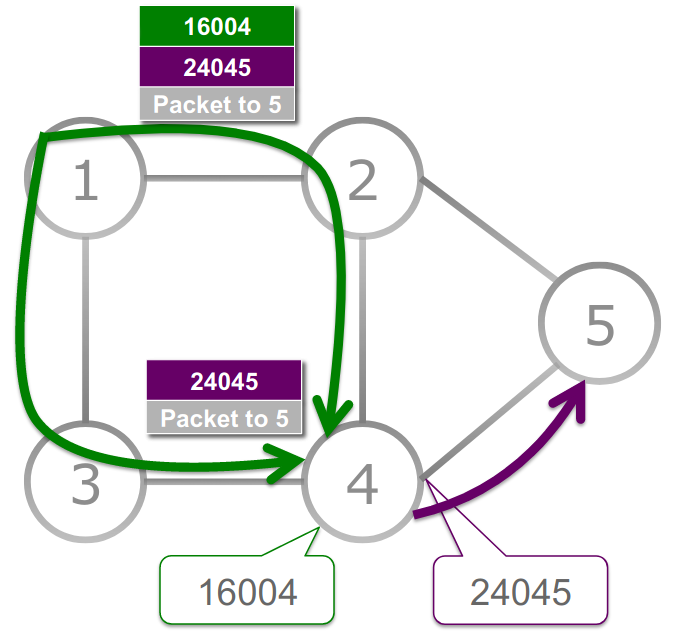
\includegraphics[width=80mm]{sr-adjacency-sid.png}
    \caption{Combining IGP PRefix and Adjacency Segments}
\end{figure}

\begin{itemize}
    \item Layer-2 Adjacency can address one specific link inside a Link Aggregation Group (LAG). 
    \item Group Adjacency
\end{itemize} 

\subsection{BGP Segments}
\begin{itemize}
    \item BGP Prefix Segment \\
    Global segment, associated with a BGP Prefix \\
    \emph{``steer traffic along the ECMP-aware BGP multi-path to the prefix associated with this segment”} 
    \item BGP Anycast Segment \\
    Traffic steering capabilities such as \emph{``steer traffic via spine nodes in group A”} 
    \item BGP Peer Segment \\
    Associated with BGP Peering sessions to specific neighbor \\ 
    Local segments that are signaled via BGP link-state address-family \\
    \emph{``steer traffic to the specific BGP peer node via ECMP multi-path towards that peer router”} \\
    Overrides the traditional BGP mechanism 
    \item BGP Peer Adjacency Segment \\
    \emph{``steer traffic to the specific BGP peer node via the specified interface towards that peer router”}
\end{itemize}

\noindent
Combining segments can create any kind of end-to-end path.

\noindent
\textbf{Traffic steering} only happens on source nodes to enable per-flow load balancing.

\noindent
For \textbf{traffic engineering} (see \ref{chapter:srte}) a policy defines the path (SID-List) to be used. 

\subsection{Labelling defaults}
Label space of Segment Routing capable software is usually reserved, even if Segment Routing is not enabled:

\begin{itemize}
    \item Label range [0-15] reserved for special-purposes
    \item Label range [16-15,999] reserved for static MPLS labels
    \item Label range [16,000-23,999] preserved for Segment Routing (Global Block)
    \item Label range [24,000-max] used for dynamic label allocation (SR Local labels)
\end{itemize}

\subsection{MPLS Data Plane}
MPLS data plane allows for direct mapping of key functionalities:

\begin{itemize}
    \item $Segment \rightarrow Label$
    \item $Segment List \rightarrow Label Stack$
\end{itemize}

\noindent
Penultimate Hop Popping is enabled by default,
Explicit-Null can be enabled if needed.

\vspace{5mm}
\noindent
Prefix-SID label is imposed on a packet if
\begin{itemize}
    \item Destination matches on a FEC (Forwarding Equivalence Class) with a Prefix-SID
    \item Downstream Neighbor is SR-Enabled
    \item Node is configured to prefer SR label imposition
    \item The matching FEC does not have an associated LDP label
\end{itemize} 

\noindent
MPLS services can be transported over SR-MPLS, removing the need for LDP as an additional protocol to operate.  

\vspace{5mm}
\noindent
Verification commands include
\ttfamily
\begin{itemize}
    \item show cef 10.0.0.1/32
    \item show cef vrf RED 10.0.0.0/30
    \item show mpls forwarding
    \item show mpls forwarding labels 16004 
\end{itemize}
\rmfamily